\chapter{Samples CuSn}
\label{chap:appendix}
\textit{}
\vfill
\minitoc
\newpage

\allowdisplaybreaks
\section{Importance to study}
\section{Sample Descriptions}

\newcolumntype{C}{>{\centering\arraybackslash}p{80mm}}% a centered fixed-width-column
\begin{table}[H]
	\centering
	\begin{tabular}{lC}
		\hline
		\hline
		&  Description\\
		\hline
		1 SLM &  CuSn / Polymer (1cmx2.5xm)\\
		2 SLM &  CuSn / Polymer (1cmx2.5xm) \\
		3 SLM &  CuSn / Polymer (1cmx2.5xm) \\
		4 SLM &  CuSn / Polymer (1cmx2.5xm) \\
		1 SLM+PP &  CuSn / Polymer (1cmx2.5xm) \\
		2 SLM+PP &  CuSn / Polymer (1cmx2.5xm) \\
		3 SLM+PP &  CuSn / Polymer (1cmx2.5xm) \\
		4 SLM+PP &  CuSn / Polymer (1cmx2.5xm) \\
		\hline
		\hline
	\end{tabular}
	\caption{Description of4 $CuSn$ samples studied }
	\label{tab:CH 3 Section 3.1 Photodectors materials}
\end{table}

\begin{figure}
	\centering
	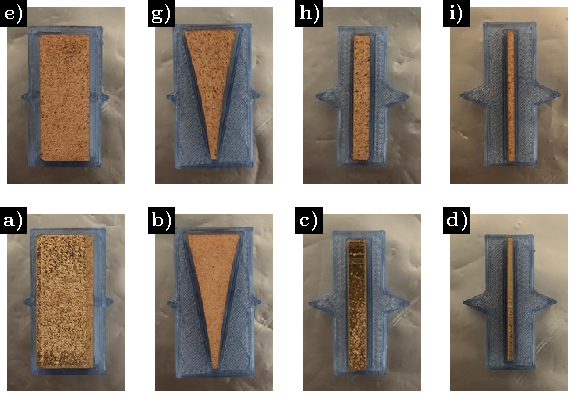
\includegraphics[width=0.8\linewidth]{FIGURES/Anexo-CuSn/table01.pdf}
	\caption{Schematic diagram of graphene properties}
	\label{fig:introfig32}
\end{figure}




\section{Results an Conclusions}



\begin{figure}
	\centering
	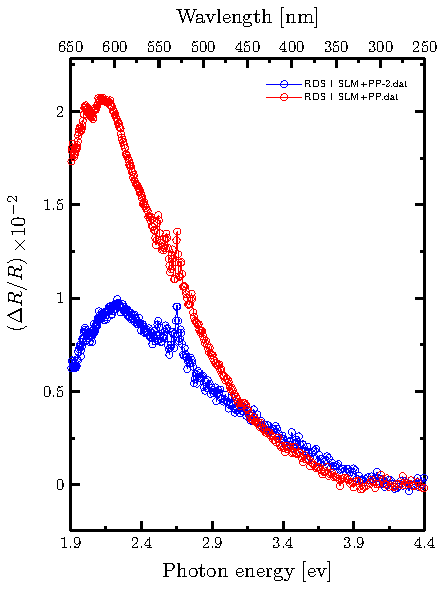
\includegraphics[width=0.5\linewidth]{FIGURES/Anexo-CuSn/RDS1SLM+PP-2}
	\caption{RDS signal for the 1SLM+PP sample in different zones.}
	\label{fig:rds-1-slmpp-2}
\end{figure}

\begin{figure}
	\centering
	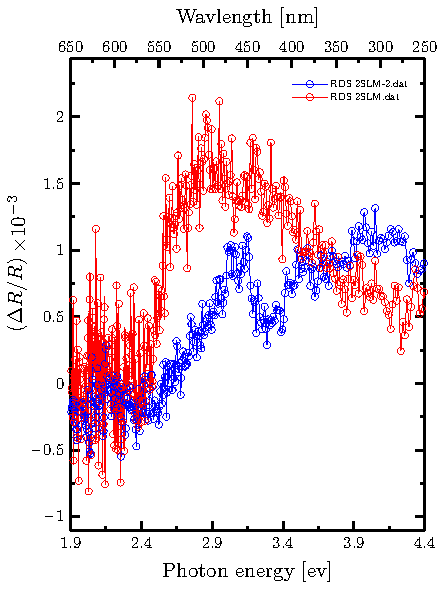
\includegraphics[width=0.5\linewidth]{FIGURES/Anexo-CuSn/RDS2SLM-2}
	\caption{RDS signal for the 2SLM sample in different zones. }
	\label{fig:rds-1-slmpp-2}
\end{figure}

\begin{figure}
	\centering
	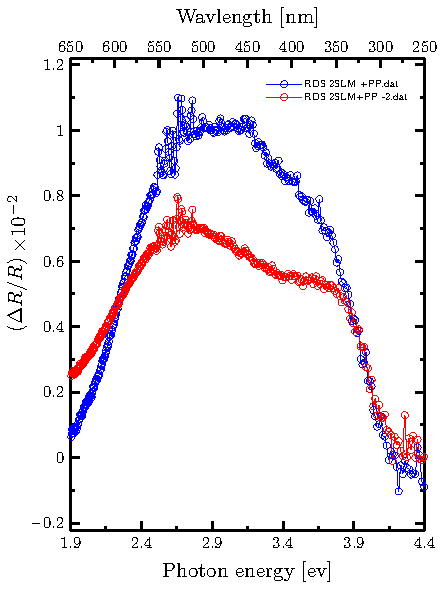
\includegraphics[width=0.5\linewidth]{FIGURES/Anexo-CuSn/RDS2SLM+PP}
	\caption{RDS signal for the 2SLM+PP sample in different zones. }
	\label{fig:rds-1-slmpp-2}
\end{figure}

\begin{figure}
	\centering
	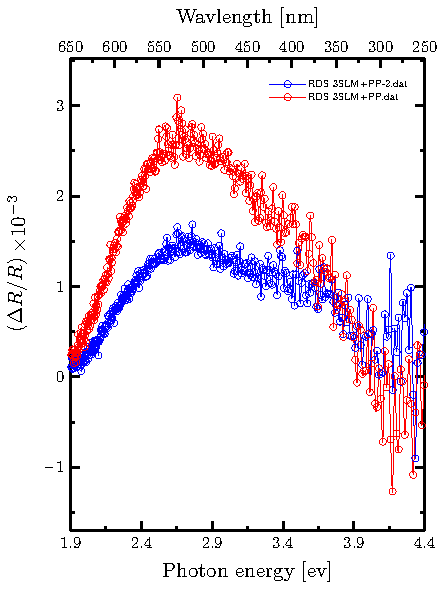
\includegraphics[width=0.5\linewidth]{FIGURES/Anexo-CuSn/RDS3SLM+PP-2}
	\caption{RDS signal for the 3SLM+PP sample in different zones. }
	\label{fig:rds-1-slmpp-2}
\end{figure}

%Resultados de las muesras de CuSb para la muestra 1SLMPP

\begin{figure}
	\centering
	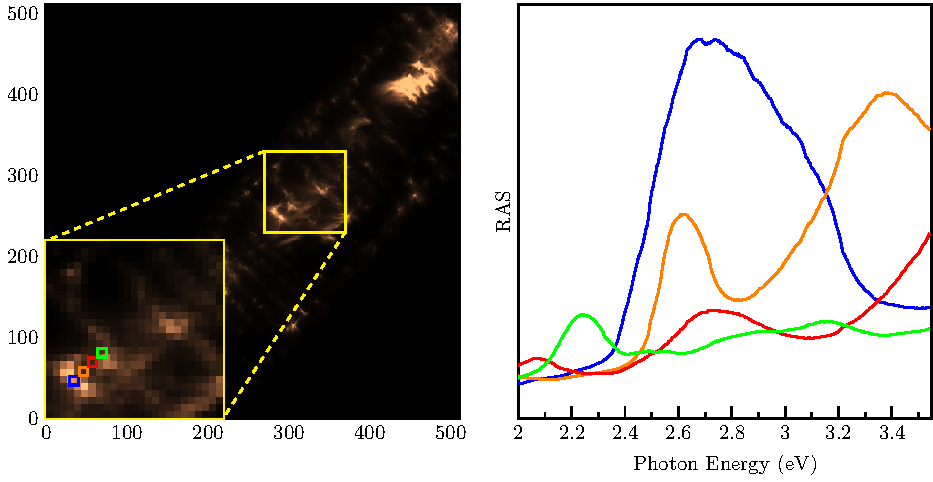
\includegraphics[width=0.8\linewidth]{FIGURES/Anexo-CuSn/1slmpp-r-0.pdf}
	\caption{Schematic diagram of graphene properties}
	\label{fig:introfig32}
\end{figure}

\begin{figure}
	\centering
	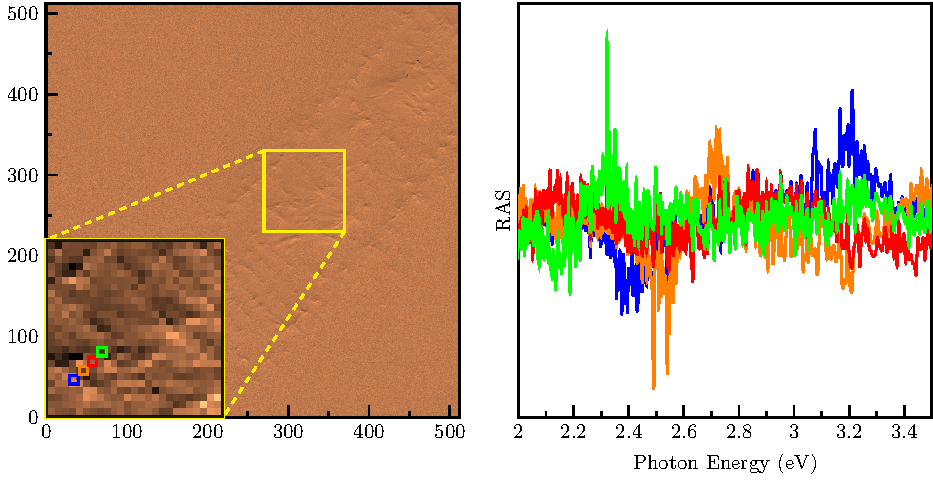
\includegraphics[width=0.8\linewidth]{FIGURES/Anexo-CuSn/1slmpp-ras-0.pdf}
	\caption{Schematic diagram of graphene properties}
	\label{fig:introfig32}
\end{figure}

\begin{figure}
	\centering
	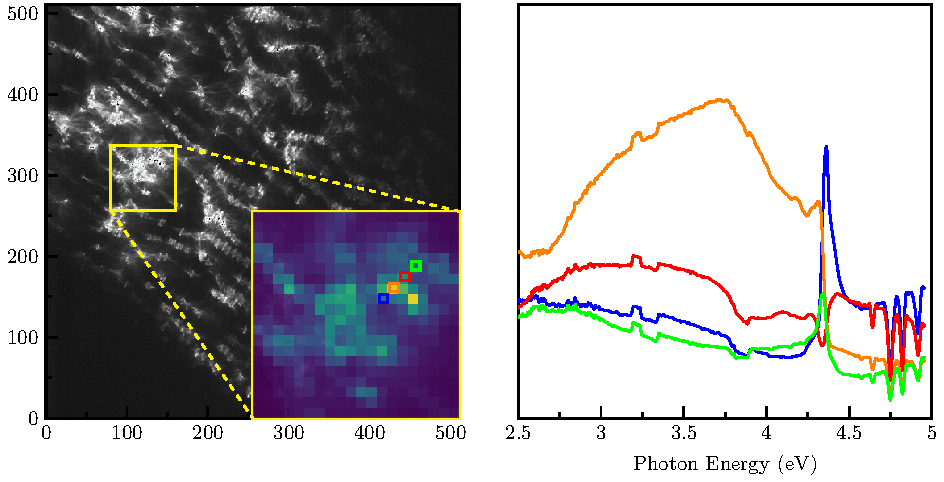
\includegraphics[width=0.8\linewidth]{FIGURES/Anexo-CuSn/2slmpp-0.pdf}
	\caption{Schematic diagram of graphene properties}
	\label{fig:introfig32}
\end{figure}


%Resultados de las muesras de CuSb para la muestra 2SLMPP

\begin{figure}
	\centering
	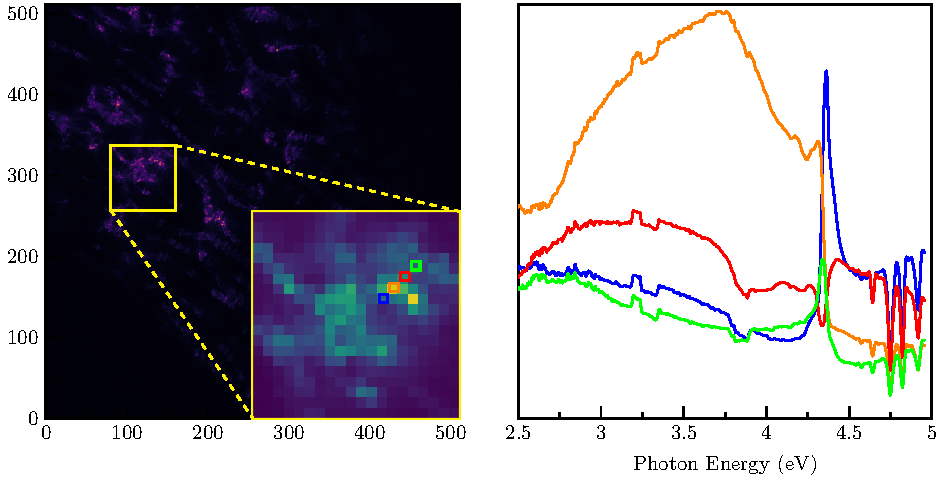
\includegraphics[width=0.8\linewidth]{FIGURES/Anexo-CuSn/2slmpp-r-0.pdf}
	\caption{Schematic diagram of graphene properties}
	\label{fig:introfig32}
\end{figure}

\begin{figure}
	\centering
	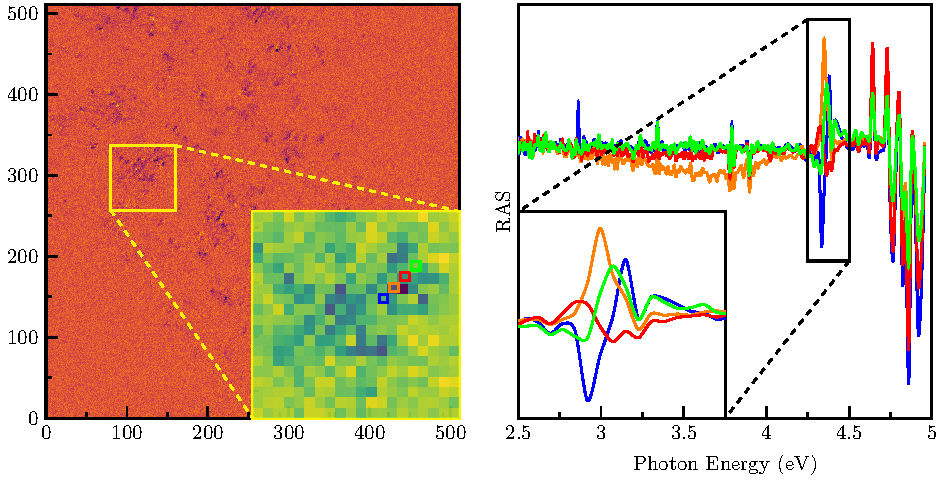
\includegraphics[width=0.8\linewidth]{FIGURES/Anexo-CuSn/2slmpp-ras-0.pdf}
	\caption{Schematic diagram of graphene properties}
	\label{fig:introfig32}
\end{figure}

\begin{figure}
	\centering
	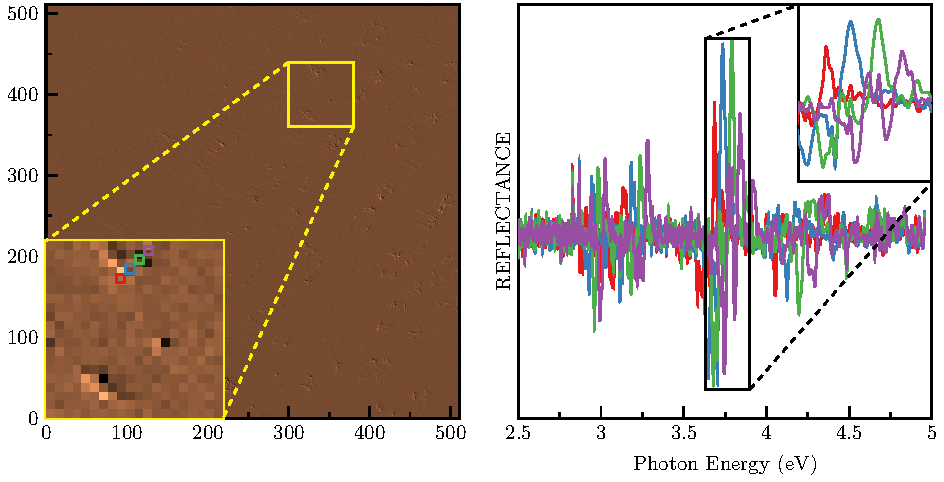
\includegraphics[width=0.8\linewidth]{FIGURES/Anexo-CuSn/2slmpp-ras-1.pdf}
	\caption{Schematic diagram of graphene properties}
	\label{fig:introfig32}
\end{figure}